\chapter{Vehicle modelling and parameterisation}\label{cha:Vehicle}

% Propulsion
\section{Propulsion} \label{sec:Propulsion}

The biggest impact of vehicle design on the trajectory is the thruster selection. As briefly outlined in \autoref{sec:Spacecraft}, the preliminary design specified a thermal arcjet and four pulsed plasma thrusters, all of which were developed within the IRS. 

A number of laboratory test results for the PPTs are reproduced in \autoref{sec:PPT-characteristics}. The test apparatus is shown in \autoref{fig:PPT}. By varying the power supplied to the PPTs, different levels of thrust were achieved for a small sacrifice in $I_{sp}$. As can be seen in \autoref{tab:PPT-performance}, increasing the power supplied to the thruster increases the mass of propellant that is vapourised and then accelerated. This increases the thrust, but the greater mass is not accelerated as efficiently resulting in a lower exhaust velocity, and consequently a lower specific impulse. 

\begin{figure}
\caption{SIMPLEX PPT during a laboratory test. The spark plug (centre left) ignites an arc between the two electrodes (pointing towards the camera) which vapourises the surface of the block of white PTFE between them. The electric field between the two electrodes then accelerates the plasma towards the camera.} \label{fig:PPT}
\centering
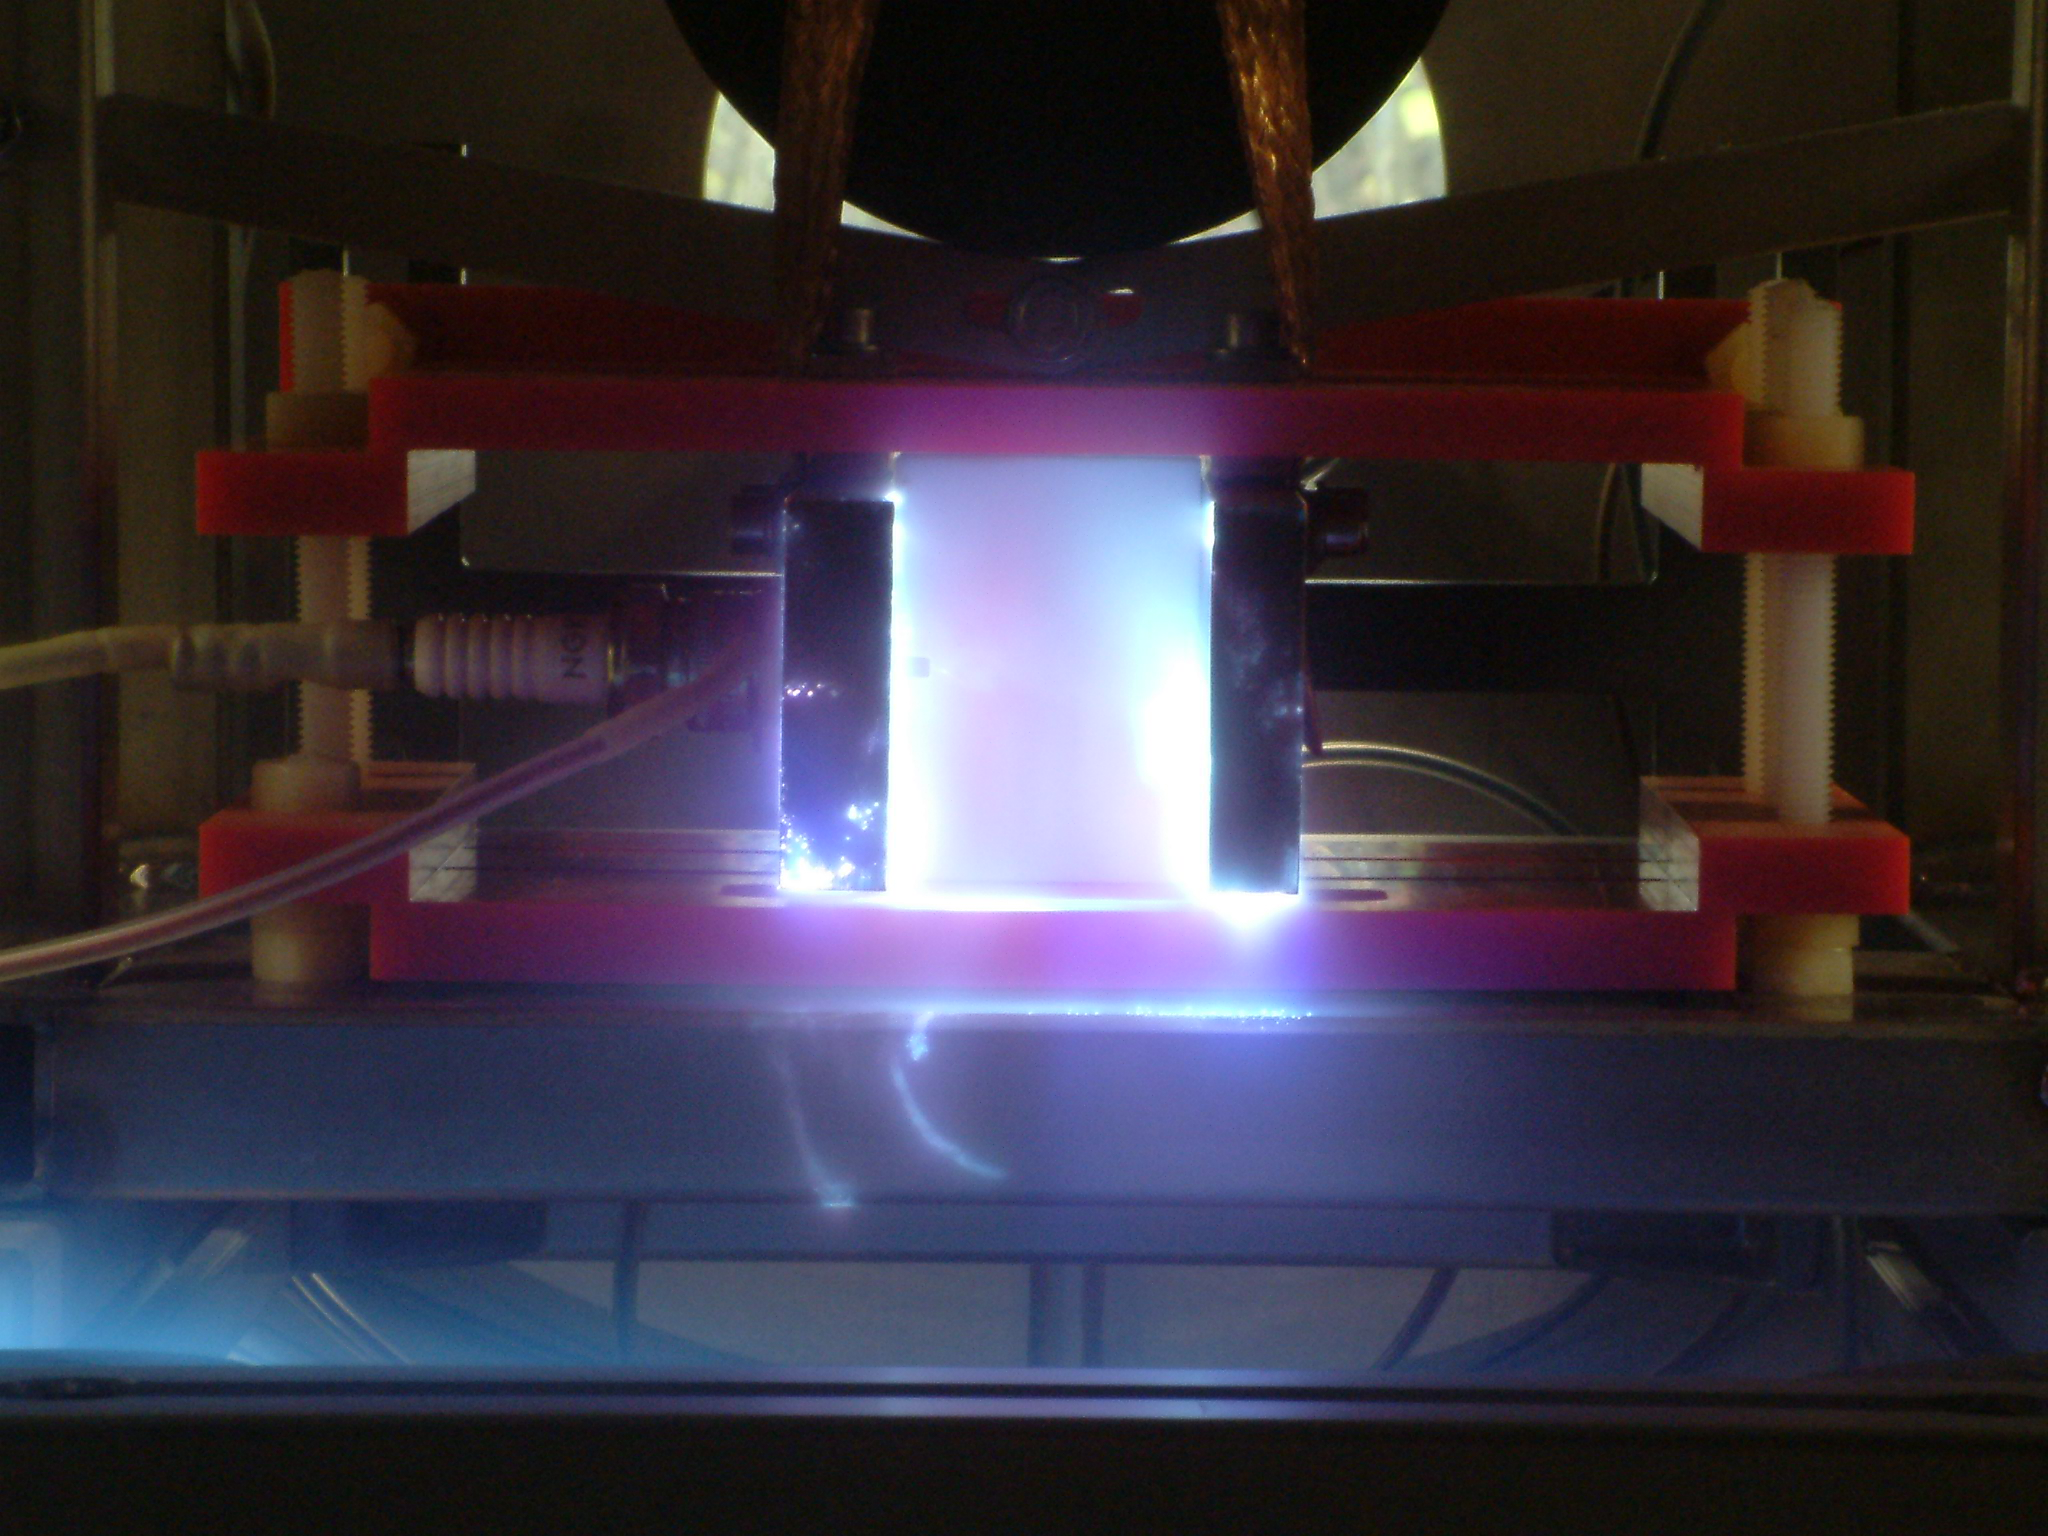
\includegraphics[width=0.7\textwidth]{Images/PPT_test.JPG}
\end{figure}

The thermal arcjet, shown in \autoref{fig:Arcjet}, underwent similar testing. The results provided to the author are reproduced in \autoref{sec:Arcjet-characteristics}. There are many more variables affecting the arcjet performance, mostly not listed in the table, but the biggest difference to the PPTs is that the rate at which propellant is provided to the arcjet can be varied independently of the power. 

\begin{figure}
\caption{TALOS arcjet during a laboratory test. An arc is generated between the axial cathode and the nozzle anode, which heats up the ammonia, accelerating it outwards.} \label{fig:Arcjet}
\centering
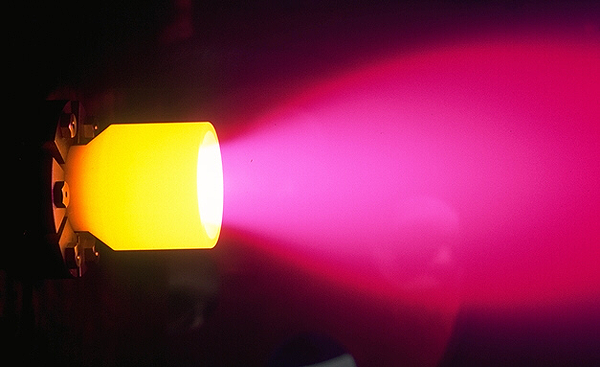
\includegraphics[width=0.7\textwidth]{Images/hiparc_betrieb.png}
\end{figure}

The thruster development at the time of writing  is focussed on improving power efficiency. The power efficiency, defined in equation \eqref{eq:thruster-efficiency}, is proportional to the thrust squared, and inversely proportional to the mass flow. Since the thrust, defined in equation \eqref{eq:thrust}, is directly proportional to mass flow, reducing mass flow will not improve power efficiency \parencite{Wollenhaupt2011}. Indeed, based on this criterion some of the arcjet tests found that the power efficiency is highest when the arc is not operated, and the thruster functions purely as a cold gas jet! 

\begin{subequations}
\begin{gather}
\eta = \frac{T^2}{2\dot{m}P} \label{eq:thruster-efficiency}\\
T = v_e\dot{m} \label{eq:thrust} 
\end{gather}
\end{subequations}

Counter-intuitively given the above definition, during testing the power efficiency often improves at the expense of thrust. This is a cause for concern, as the low thrust has already required a much longer transfer than any used in the past, and the longer the mission the greater the chance of impact with space debris or micrometeorites, damage from radiation, or computer failure due to solar proton events (SPEs) or galactic cosmic rays (GCRs).

Furthermore, the length of the cruise phase frequently resulted in computational difficulty, so a number of design compromises were investigated to solve the problem (it is acknowledged by the author that changing hardware design to make the simulation easier is a poor design philosophy, but the project management was interested to know the effects of these changes regardless of any simulation difficulties). For example, a design configuration was being investigated with 6 PPTs rather than 4, thereby increasing the available thrust without losing $I_{sp}$. The trade-off with this change is the additional thrusters would increase the dry mass of the vehicle, decreasing available payload space. The same effect could be achieved by changing the pulse rate of the PPTs. A higher pulse frequency increases thrust, increases mass flow, and increases power consumption, but impulse is conserved. However, an additional unknown is introduced: the heat flux within the electrodes is increased. 

% Thrust and power can also be linearly scaled by simply introducing more PPTs to the structure. This has been championed by the PPT designer, Matthias Lau. This option increases the redundancy of the system (and therefore reliability). However, it also carries the associated cost of extra weight.

Increasing the heat generated by the PPTs causes a corresponding increase in the electrodes operating temperature, until a new equilibrium is reached with the heat radiated into space. This higher temperature can cause damage to the electrodes, structural failure in the surrounding satellite components, or even melt the propellant! There is literature indicating that some designs can tolerate higher pulse frequencies \parencite{Mueller2000} but the majority of documented laboratory tests use 1~Hz. Consequently, thorough lifecycle testing will be required on the thrusters to determine operational lifetime variability with pulse frequency before a 4 year mission such as \BW\ may be undertaken. 

% From the power output, realised that the design could use more power to transfer faster - take many forms. Higher pulse frequency most promising, this linearly increases thrust at exactly the same Isp, at the cost of linearly increasing power consumption. The only limitation is wear and tear to the service life of the thruster; should be proportional to the number of pulses and since each pulse provides a certain Impulse bit, the number of pulses required to perform the lunar transfer should be constant. Thrusters have not been endurance tested yet meaning we don't know how many cycles they can perform. Other constraint is cooling - over about 3~Hz the PTFE is not able to cool properly between cycles and can interfere in the thruster performance. However, some tests performed in Russia (cite Matthias and/or Pedro here?) have successfully used a design similar to SIMPLEX at 20~Hz.

% Finally, extra power can be discharged into each pulse. This increases the Isp and thrust because the plasma is accelerated faster, but the increase is not proportional to the extra power put into each pulse. Therefore the power efficiency drops. Currently the development of the PPTs is focussed on improving the power efficiency, so the performance at this opposite end of the scale is not well characterised/not well known.

Nonetheless, when modelling the PPTs an additional variable was implemented representing maximum pulse frequency. Operationally, the variable thrust magnitude would be implemented by reducing the pulse frequency from the maximum available. Colleagues at IRS advised that the SIMPLEX PPT should be able to operate up to at least 3~Hz with minimal side effects \parencite{Cabrera2011}.

The first simulation implemented 4 PPTs operating at 1~Hz for the cruise phase. This implementation took 2298~radians $\Delta L$ and about 950~days to ascend to the phase boundary. Optimisation was not possible due to numerical limitations. Given the surplus power available at all stages of this ascent, it was run again at 2~Hz. This second simulation took 1347~radians and about 500~days to ascend to the phase boundary. Based on the discretisation philosophy outlined in \autoref{sec:Parameterisation}, this almost halved the number of optimisable parameters. 

% regardless, it was found that increasing the thrust shortens the transfer but makes lunar capture more difficult. The higher thrust may be targeted at the Moon, and an appropriate orbital energy can be attained for lunar capture (about 5000~m$^2$s$^{-2}$) but due to the higher thrust, a larger proportion of the energy is made up of kinetic energy. In other words, the spacecraft is going too fast to achieve a strong lunar capture, even with a very low lunar pass. Perhaps relative velocity might be a better termination criterion?


%-----------------------------------------------------------------------------------------------------------------------------------------------

% Earth shadow
\section{Earth shadow}

During the transfer, the spacecraft may be eclipsed by the Earth or the Moon. When either of these large bodies are blocking the Sun, the spacecraft does not gain any charge to its solar panels, and is unaffected by solar wind. 

The occlusion of a luminous sphere by a smaller sphere creates a conical shadow called the \emph{umbra}, as shown in \autoref{fig:Eclipse}. Within the umbra a total eclipse is observed. Surrounding the umbra is an inverted cone of partial shadow called the \emph{penumbra}. An observer within the penumbra would experience a partial eclipse. Beyond the umbra is another inverted cone of partial shadow called the \emph{antumbra}, within which an annular eclipse would be observed \parencite{Longo1995}.

\begin{figure}
\caption{Umbra, penumbra and antumbra.} \label{fig:Eclipse}
\centering
\def\svgwidth{0.85\textwidth}
\input{Images/eclipse-1.pdf_tex}
%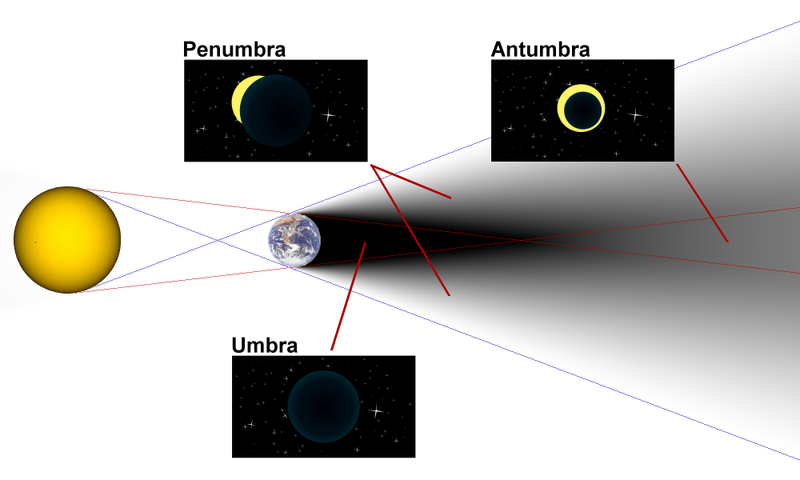
\includegraphics[width=\textwidth]{Images/eclipse.png}
\end{figure}

First the apices and lengths of the cones may be determined using the simple geometry shown in \autoref{fig:Umbra} and \autoref{fig:Penumbra} giving equation \eqref{eq:cones}.
\begin{subequations} \label{eq:cones}
\begin{gather}
\alpha_u = \arcsin\frac{R_\Sun-R_\Earth}{r_\Earth} \\
\alpha_p = \arcsin\frac{R_\Sun+R_\Earth}{r_\Earth} \\
x_u = \frac{R_\Earth r_\Earth}{R_\Earth-R_\Sun} \\
x_p = \frac{R_\Earth r_\Earth}{R_\Earth+R_\Sun}
\end{gather}
\end{subequations}
where $\alpha_u$ is the apex angle of the umbral cone and $\alpha_p$ is the apex angle of the penumbral cone, $x_u$ is the length of the umbral cone and $x_p$ is the length of the penumbral cone, $R_\Sun$ is the radius of the Sun and $R_\Earth$ is the radius of the Earth, and $r_\Earth$ is the distance between the Earth and the Sun.

\begin{figure}
\caption{Umbral cone.} \label{fig:Umbra}
\centering
\def\svgwidth{0.6\textwidth}
\input{Images/eclipse-2.pdf_tex}
%\reflectbox{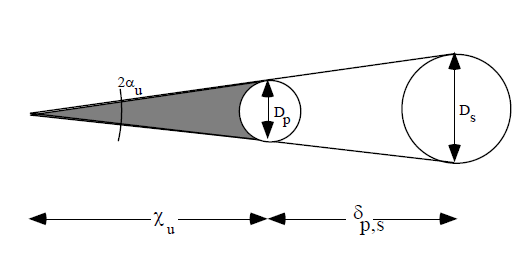
\includegraphics[width=\textwidth]{Images/umbra.png}}
\end{figure}

\begin{figure}
\caption{Penumbral cone.} \label{fig:Penumbra}
\centering
\def\svgwidth{0.6\textwidth}
\input{Images/eclipse-3.pdf_tex}
%\reflectbox{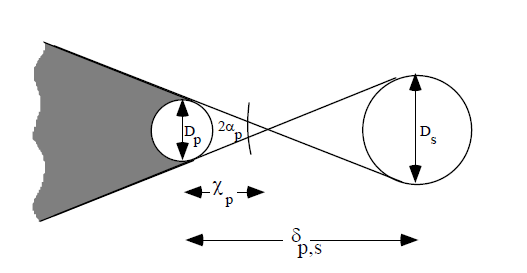
\includegraphics[width=\textwidth]{Images/penumbra.png}}
\end{figure}

%Next a fundamental plane is defined through the centre of the Sun and the spacecraft, perpendicular to the plane including the Sun, spacecraft and planet.
%First the distance between the occluding body and the fundamental plane is calculated.
%First the position vector of the spacecraft relative to the central body is projected onto the fundamental plane.
The spacecraft's position is then projected onto the Earth-Sun vector, and the satellite's distance from the Earth-Sun line is calculated using the geometry shown in \autoref{fig:Spacecraft-shadow}.
\begin{subequations}
\begin{gather}
x = \frac{\vec{r}\cdot\vec{r_\Earth}}{|\vec{r_\Earth}|} \\
y = \sqrt{|\vec{r}|^2-x^2} 
\end{gather}
\end{subequations}

\begin{figure}
\caption{Spacecraft position relative to Earth-Sun line.} \label{fig:Spacecraft-shadow}
\centering
\def\svgwidth{\figurewidth}
\input{Images/eclipse-4b.pdf_tex}
%\includegraphics[width=\textwidth]{Images/earth-shadow.png}
\end{figure}

Now the radii of the umbral cones at the satellite's position may be calculated.
\begin{subequations}
\begin{gather}
y_u = (x_u-x)\tan\alpha_u \\
y_p = (x+x_p)\tan\alpha_p
\end{gather}
\end{subequations}

Within this frame, if the spacecraft's position $y$ is less than the radius of the umbral cone $y_u$, the spacecraft experiences total eclipse. If the spacecraft's position is more than the radius of the penumbral cone $y_p$, the spacecraft is in full sunshine. For simplicity, solar exposure within the penumbra was taken as a simple linear interpolation of position $y$ between the umbral and penumbral cones. During lunar-centric phases the same equations apply but with the spacecraft's position relative to the Moon $r_\Moon$ rather than the Earth $r_\Earth$.

% Antumbra?
% If closer to the Sun than the central body?

% Power
\section{Power}\label{sec:Vehicle-power}

\subsection{Power generation} \label{sub:Power-generation}

At the commencement of this project, it was anticipated that power would be one of the defining factors in determining an optimal trajectory. Consequently power was implemented as one of the states to be tracked during optimisation. The power generation was calculated using equation \eqref{eq:Power-generation},
\begin{gather} \label{eq:Power-generation}
P = Q\times A_{eff}\times\eta_a\times\eta_c\times\eta_{DC}\times\cos\Psi_\Sun\times\mathfrak{R}
\end{gather}
where $Q$ represents the solar energy flux near the Earth-Moon system, $\eta_a$ represents the area efficiency of the solar cells arranged within the panel, $\eta_c$ represents the solar cell efficiency, and $\eta_{DC}$ represents the efficiency of the voltage regulator. The angle subtended by the sun on the solar panels is $\Psi_\Sun$, and the power degradation is $\mathfrak{R}$.

The solar energy flux is calculated by dividing the average solar luminosity \parencite[$3.846\times10^{26}$ W,][]{Montenbruck2000} by the surface area of a sphere with radius equal to the spacecraft's distance from the Sun ($4\pi r_\Sun^2$). This is important because the Earth's distance from the Sun varies by 6\% over the year \parencite{Montenbruck2000} due to the eccentricity of its orbit. The solar intensity is then multiplied by the effective area of the solar panels, $A_{eff}$. Although the spacecraft has 6~m$^2$ of panels, because the central two panels are positioned at 45\degrees\ the effective area is only 5.4~m$^2$.

Based on the latest design work by my colleague Alexander Uryu, the area efficiency is about 0.8, that is, only 80\% of the effective solar panel area will actually be covered in solar cells, due to the geometric arrangement of the cells and the additional surface area required for circuitry. The solar cells will be state-of-the-art TEC-STAR GaAs/InP 34 series solar arrays with 200~$\mu$m front cover glass and 500~$\mu$m back cover glass. Consequently it is estimated that the cell efficiency will be about 27\% at launch. The exact power control circuitry is not yet known, but based on modern power conversion ciruits it is expected that the DC voltage regulator will be approximately 85\% efficient. 

It is assumed that while one axis of the solar panels is constrained to the thrust vector $\vec{u}$, the other is free to rotate about the thrust vector to obtain the best sun angle possible. Consequently the sun angle can be calculated using equation \eqref{eq:sun-angle}.
\begin{subequations}
\begin{gather} \label{eq:sun-angle}
\vec{u}\cdot\vec{r}_\Sun = |\vec{u}|.|\vec{r}_\Sun|\cos\Psi \\
\Psi = \arccos\frac{\vec{u}\cdot\vec{r}_\Sun}{|\vec{u}|.|\vec{r}_\Sun|}
\end{gather}
\end{subequations}

The greatest unknown in the power model is how much the solar cells will degrade over time. As \textcite{Erb_thesis} points out, the solar panel degradation, $\mathfrak{R}$, is directly related to total equivalent \emph{fluence}, $\mathfrak{F}$ (that is, the radiation dose received), which must be integrated over the transfer, where the derivative with respect to time $\frac{d\mathfrak{F}}{dt}$ is approximated as a function of the distance from Earth, as shown in \autoref{fig:Fluence}. 

\begin{figure}
\caption{Radiation fluence during a 24 hour orbit as a function of distance from Earth.} \label{fig:Fluence}
\centering
\def\svgwidth{\figurewidth}
\input{Images/fluence.pdf_tex}
\end{figure}
  
At each time step the equivalent radiation dose of a 24~hour orbit may be taken from the graph, and scaled to the appropriate time interval. This effective radiation dose is added to the accumulated radiation dose. The total accumulated radiation dose may be translated to a power degradation factor using \autoref{fig:Fluence2}.

\begin{figure}
\caption{Power degradation as a consequence of radiation fluence.} \label{fig:Fluence2}
\centering
\def\svgwidth{\figurewidth}
\input{Images/fluence2.pdf_tex}
\end{figure}

Data for the panel degradation model was based on the work done by \textcite{Hechler2002} during planning for the SMART-1 mission, via \textcite{Erb_thesis}. During the SMART-1 mission, it was found that their solar cells degraded by approximately 0.12\% per day, or about 2~W \parencite{Racca5}. It was also found that during a solar storm on 20~October 2003, an additional 1\% panel degradation occurred \parencite{Racca8}. However, soon after the solar storm, the spacecraft reached a periapsis of 11790~km whereupon no further radiation damage occurred. Thus it can be assumed that the phase boundary defined in the mission architecture may be quite conservative, which should be factored into further power degredation modelling if not simply changing the mission architecture.

% optimisable fixed-body thrust vector allows trade-off between thrust angle and solar panel orientation - if the craft isn't thrusting, it can still use the thrust vector controls to point the solar panels at the sun

\subsection{Power consumption} \label{sub:Power-consumption}

At each timestep the power required for communications, payload and thrust would be subtracted from the power generated. 

The payload has not yet been confirmed, but it is expected that most of the payload will be in standby until the spacecraft is confirmed in the science orbit, so power requirements during the transfer will be minimal. During the science phase the payload is expected to require approximately 300~W \parencite{web_BW-1}, which should be well within the solar panels' remaining capacity.

Agreements are being negotiated with ground stations in Stuttgart, USA, Japan and Australia to give continual access to the satellite during Earth orbit. The only downtime will occur in the later stages of the transfer, when the satellite transits through the Moon's shadow. Access time notwithstanding, the satellite will have to rotate to point its antennae towards the Earth during transmission. Therefore it is expected that communications will only operate a fraction of the transfer time. These communications intervals will be scheduled based on availability of both power and coasting phases, and as such should not impact the trajectory design. During communications intervals approximately 250~W will be required for the Ka-band transmission, and 10~W for the S-band.

After thruster power is also subtracted from generated power (see \autoref{sec:Propulsion}), any surplus power generated by the solar panels is added to the battery levels, or any deficit is subtracted from them. According to the initial design stated by \textcite{Falke2004}, the lithium ion batteries were designed to hold 100~Ah supplying a common bus of 28~V. It is assumed the batteries will be fully charged at launch. At any stage during the transfer, if the batteries become fully charged the spacecraft will roll around its thrust vector to point the solar panels away from the Sun, thus preventing overcharge.

%-----------------------------------------------------------------------------------------------------------------------------------------------

% Parameterisation
\section{Parameterisation} \label{sec:Parameterisation}

\subsection{Substitution of parameters}\label{sub:subst-param}
\autoref{sec:state-vector} establishes the state vector $\vec{x}=\{p,f,g,h,k,L,m,t,E\}$, and provides the differential equations with respect to time. However, as outlined in \autoref{sec:Independent-parameter}, the normalised true anomaly, $Ln$, was the independent parameter. Therefore a subsitution of parameters is required to give derivatives with respect to $Ln$, $\frac{d}{dLn}$. Differentiating equation \eqref{eq:Ln} results in \eqref{eq:dLndt},
\begin{subequations} \label{eq:dLndt}
\begin{gather}
\frac{dLn}{dt}=\frac{1}{\Delta L}\frac{dL}{dt} \\
\frac{dLn}{dt}\cdot\frac{dt}{dL}=\frac{1}{\Delta L} \\
\frac{dLn}{dL}=\frac{1}{\Delta L} \\
\frac{dL}{dLn}=\Delta L
\end{gather}
\end{subequations}

Using this identity, the state differential equations with respect to normalised longitude \eqref{eq:dpdLn} may be determined.
\begin{subequations}\label{eq:dpdLn}
\begin{align}
\frac{dp}{dLn}&=\frac{dp}{dt}\cdot\frac{dt}{dLn}\\
&=\frac{dp}{dt}\cdot\frac{dt}{dL}\cdot\frac{dL}{dLn}\\
&=\frac{\dot{p}}{\dot{L}}\Delta L
\end{align}
\end{subequations}

%The differential equations for $f$, $g$, $h$, $k$ and $m$ are modified similarly to $p$. $L$ is simply $\frac{dL}{dLn}$. Substituting the parameters of the remaining differential equations gives:
%\begin{subequations}
%\begin{align}
%\frac{dt}{dLn}&=\frac{dt}{dL}\cdot\frac{dL}{dLn}\\
%&= \frac{1}{\dot L}\cdot\Delta L
%\end{align}
%\end{subequations}
%\begin{subequations}
%\begin{align}
%\frac{dE}{dLn} &= \frac{dE}{dt}\cdot\frac{dt}{dL}\cdot\frac{dL}{dLn} \\
%&= \frac{P}{\dot{L}}\cdot\Delta L 
%\end{align}
%\end{subequations}
The remaining differential equations are modified similarly. The final equations are presented in \eqref{eq:dLn},
\begin{subequations} \label{eq:dLn}
\begin{gather}
\frac{dp}{dLn}=\frac{\dot{p}}{\dot{L}}\Delta L \\
\frac{df}{dLn}=\frac{\dot{f}}{\dot{L}}\Delta L \\
\frac{dg}{dLn}=\frac{\dot{g}}{\dot{L}}\Delta L \\
\frac{dh}{dLn}=\frac{\dot{h}}{\dot{L}}\Delta L \\
\frac{dk}{dLn}=\frac{\dot{k}}{\dot{L}}\Delta L \\
\frac{dL}{dLn}=\Delta L \\
\frac{dm}{dLn}=\frac{\dot{m}}{\dot{L}}\Delta L \\
\frac{dt}{dLn}=\frac{1}{\dot{L}}\Delta L \\
\frac{dE}{dLn}=\frac{P}{\dot{L}}\Delta L 
\end{gather}
\end{subequations}
where $\dot{p}$, $\dot{f}$,  $\dot{g}$, $\dot{h}$, $\dot{k}$ and $\dot{L}$ are the original time-domain differential equations provided by \textcite{Walker1985}.

\subsubsection{Delta-v calculation}
The universal definition for delta-v was provided in \autoref{sub:Delta-v}. Unfortunately this definition also depends on time-domain integration. Therefore another substitution of parameters is required.
\begin{subequations}
\begin{align}
\Delta v &= \int^{Ln_f}_{Ln_i}\frac{|T|}{m}\frac{\text{dt}}{\text{dLn}}\text{dLn}\\
&= \int^{1}_{0}\frac{|T|}{m}\frac{\text{dt}}{\text{dL}}\cdot\frac{\text{dL}}{\text{dLn}}\text{dLn}\\
&= \int^{1}_{0}\frac{|T|}{m}\frac{\Delta L}{\dot L}\text{dLn}
\end{align}
\end{subequations}


\subsection{Thrust profile parameterisation} \label{sub:Thrust-parameterisation}

% Departure date
Due to the particularly non-linear variations with departure date (periodic over 27.5~days based on the Moon's orbit) a good parameterisation of the departure date would be to use two variables, one to increment an integer number of lunar months forwards or backwards, the other a floating point capped at $\pm 0.5$ to indicate the fraction of a month either side. This allows the optimiser to find the optimal time of month for a launch, and therefore the optimal position of the Moon, to achieve lunar capture. Then the optimiser can adjust the month forwards or backwards based on other variations in the search space. While this parameterisation would assist in developing a truly optimal solution, since the departure date is not negotiable beyond the time spent in the GTO parking orbit it was not implemented at this time.

% Thrust duty cycle
An additional parameterisation considered to decrease the numerical complexity of the optimisation is to model the thrust duty cycle as a percentage of the orbit. Depending on the phase objective, a thrust segment was centred around the periapsis or apoapsis, with a parameter controlling for which percentage of the orbit the thrusters were active. However, when implemented as a constant throughout the phase replacing the continuous thrust magnitude, the optimiser's flexibility is severely compromised. When implemented as a constant throughout the phase in addition to the thrust magnitude parameter, there is no improvement in computational load. An alternative would be to implement duty cycle as a continuous variable. The computational load is just as great, but the author suspects that this modification would significantly smooth the search space. Unfortunately, due to the complications experienced when optimising the system with a continuous thrust magnitude parameter this modification was not trialled.


\subsection{Discretisation} \label{sub:Discretisation}
As mentioned in \autoref{sec:Process}, numerical solution methods require the continuous state and control profiles to be discretised into a series of grid points or nodes. GESOP allows these grid points to be distributed arbitrarily over the independent parameter, although given the number of grid points required for low thrust transfers and how the shape of the trajectory can change during optimisation anything other than a uniform distribution makes no sense.

As mentioned in \autoref{sec:Independent-parameter}, longitude was selected as the independent parameter to allow equiangular node distribution. As a rule of thumb, for the initial coarse mesh at least 10~grid points were implemented for each orbit. As a result, the cruise phase had over 7300~grid points. Later in the project an automatic mesh generator was implemented in GESOP. Using this mesh generator based on an error tolerance of $1.0\times10^4$ gave a starting baseline of 20003~grid points for the cruise phase. 

Within each of these shooting intervals, a finer mesh of control nodes may be specified. Multiple shooting methods allow the state and control profiles to be approximated over each of these sub-intervals as a piecewise polynomial function. Thus, with enough control nodes, the state and control profiles appear almost continuously variable. Single shooting methods use only the major nodes, and ignore the control refinement mesh. Constraint violations are evaluated at each shooting node, although GESOP once again allows a finer mesh to be specified by the user. However, SOCS does not support additional constraint evaluations, and as a single shooting method it ignores the control refinement mesh.

Nonetheless, during optimisation the major control mesh undergoes repeated refinement until the optimisation and errors are within user-defined tolerances. At the time when the cruise phase optimisation was stopped (see \autoref{sec:Cruise}), the mesh had been refined to 99979~grid points. The ascent phase also started from 20003 grid points and was refined to 29999~points by the time it found a feasible solution with a targeted optimisation tolerance of $10^{-4}$, constraint tolerance of $10^{-5}$ and ODE tolerance of $2\times10^{-5}$. For comparison, the reduced complexity ascent phase (see \autoref{sec:Reduced-complexity}) was started from 1002~grid points, and reached 13990~points by the time it found an optimal solution.

% ascent2 - initial guess 1000 grid points, opt tolerance 1.0e-4, constraint tolerance 1.5e-8, ode tolerance 1.0e-7, 10 mesh refinements, 2000 iterations, hermite simpson separate method, 8e7 real workspace, 4e7 integer
% 1002 initi guess, 13990 optimised

% ascent - automatic mesh generation, opt tolerance 1.0e-4, constraint tolerance 1.0e-5, ode tolerance 2.0e-5, 5 mesh refinements, 5 iterations, hermite simpson separate method, 25e7 real workspace, 8e7 integer 
% 20003 initi guess, 29999 feasible

% cruise - automatic mesh generation, opt tolerance 9.0e-4, constraint tolerance 1.0e-5, ode tolerance 2.0e-5, 5 mesh refinements, 5 iterations, hermite simpson separate method, 20e7 real workspace, 8e7 integer 
% 20003 initi guess, 99979 semi-feasible

% MERELY PROPAGATION
% propagate - automatic mesh generation, integration error 1.0e-8, minimum 10000 output points to generate a smooth image

% NOT OPTIMISED
% capture - automatic mesh generation, opt tolerance 1.0e-7, constraint tolerance 1.5e-8, ode tolerance 1.0e-7, 10 mesh refinements, 2000 iterations, hermite simpson separate method, 8e7 real workspace, 4e7 integer 

% NOT OPTIMISED
% descent - automatic mesh generation, opt tolerance 1.0e-7, constraint tolerance 1.5e-8, ode tolerance 1.0e-7, 10 mesh refinements, 2000 iterations, hermite simpson separate method, 8e7 real workspace, 4e7 integer 

\textcite{Betts1998} provides a simple algorithm to estimate the number of variables required in a large optimsation problem, as a function of the number of states $n_x$, the number of control parameters $n_u$, the number of optimisable phases $M$ and the number of gridpoints per phase $N$.
%\begin{subequations}
\begin{gather}
n \approx (n_x + n_u)MN %\\
%n_y = 8 \\
%n_u = 4 \\
%M = 4 optimisable phases \\
%N = 80,000 grid points per phase \\
%=2.56e6 \\
\end{gather} %\end{subequations}
Given the problem formulation outlined for \BW\ in \autoref{cha:Optimisation}, just the cruise phase ends up with $1.2\times10^6$ variables, substantially more than the 500,000 cited by \textcite{ASTOS_guide} as the largest problem SOCS has solved. Consequently, running the optimisation routine on the cruise phase required $2\times10^8$ 64-bit doubles for floating point operations and $8\times10^7$ 32-bit words for integer operations. The desktop PC kindly provided by the Institute of Space Systems in Stuttgart, an AMD~2.8GHz~X6 with 2GB~RAM, was unable to handle a problem of this order. Despite an upgrade to 4GB, the optimisation was still sluggish, and consequently was terminated before it could achieve an optimal solution. 


%No DOF : number of parameters minus active constraints. Approx 50,000 for Cruise phase


%-----------------------------------------------------------------------------------------------------------------------------------------------

\section{Orbital behaviour}

Previous theoretical analysis and numerical studies have identified a number of phenomena related to orbital transfers. A description of the theory behind gravitational assists, the Oberth effect, and weak lunar capture as they relate to \BW\ is briefly presented here.

\subsection{Gravitational assists} \label{sub:Grav-assist}

Due to the low thrust of spacecraft \BW, a substantial part of the orbit raising can be achieved by exploiting the gravitational pull of the Moon. This technique has been well studied, although previous higher-thrust missions did not find it efficient to attempt more than one or two lunar resonances. \textcite{Kemble2006} explains that \enquote{It is possible to utilise lunar gravity to assist in the orbit raising prior to lunar encounter. This takes the form of a \emph{gravitational pumping} effect if the correct phase with respect to the Moon can be established}. He goes on to quantify that \enquote{A typical $\Delta V$ saving of 800~ms$^{-1}$ is obtained by use of lunar gravity assist}. 

Because lunar gravitational assists provide delta-v without fuel expenditure, they should be implicitly accounted for during optimisation. Preliminary results did indicate this to be the case, as seen in \autoref{fig:Lunar-resonance}. From an initial orbit of 180,000~km (semi-cis-lunar, representing the later stages of the transfer to highlight the lunar assist) the spacecraft takes two orbits to align its phase with the Moon, then receives a very apparent boost purely from the Moon's gravity during the close passes seen in \autoref{fig:Lunar-resonance2}.

\begin{figure}
\caption{Trajectory of preliminary optimisation showing a lunar resonance implicitly realised by the optimiser.} \label{fig:Lunar-resonance}
\centering
\def\svgwidth{\figurewidth}
\input{Images/grav-assist.pdf_tex}
\end{figure}

\begin{figure}
\caption{Distance of spacecraft from Earth and Moon during preliminary optimisation showing a lunar resonance implicitly realised by the optimiser.} \label{fig:Lunar-resonance2}
\centering
\def\svgwidth{\figurewidth}
\input{Images/grav-assist2.pdf_tex}
\end{figure}




\subsection{Oberth effect and optimal thrust profiles} \label{sub:Oberth}

It is well known that thrusting at particular points in the orbit is more efficient than others \parencite{Kemble2006}. \textcite{Oberth1923} states that the specific orbital energy gained per unit delta-v exerted is equal to the instantaneous speed. Therefore, thrusting is more efficient at high speed, which occurs at periapsis. This is known as the Oberth effect, and is demonstrated quite effectively in \autoref{fig:oberth} where the \emph{effective weight} is the weight minus the centrifugal force due to the horizontal velocity.

\begin{figure}
\caption{Thrust to effective weight ratio during preliminary optimisation demonstrates the Oberth effect.} \label{fig:oberth}
\centering
\def\svgwidth{\figurewidth}
\input{Images/oberth.pdf_tex}
\end{figure}

Constant thrust (tangential to the orbital radius) leads to circular trajectories because an eccentric starting trajectory spends more time at apoapsis than periapsis; hence more impulse is imparted to the vehicle at apoapsis than at periapsis. As evident in a Hohmann transfer, thrusting at apoapsis circularises the orbit. \textcite{Racca9} found that tangential thrust is the most efficient way to increase the periapsis of a constant-thrust vehicle.

In a vehicle with variable thrust however, the majority of the thrusting should occur near perigee; there is an inverse relationship between optimal thrust magnitude and orbital radius. However, the ascent phase of \BW\ requires raising the periapsis above the van Allen belts as quickly as possible. This may be achieved by focussing thrust around the apoapsis; unfortunately this also minimises the orbital energy gained per unit of propellant expended. Consequently, in the subsequent cruise phase once the periapsis requirement is removed and the sole aim is to gain orbital energy as efficiently as possible, it would be expected that thrust is focussed around the periapsis. \textcite{Racca9} found that the most efficient thrust profile for a constant-thrust vehicle to increase orbital energy (proportional to semimajor axis) is to thrust along the velocity vector. However, \BW\ requires some additional maneouvres during this phase. 

In addition to orbital energy and the corresponding semimajor axis, there are well established strategies for efficiently changing other orbital parameters. For example, \textcite{Edelbaum1964} demonstrates that the argument of periapsis ($\omega$) is most efficiently changed during a low eccentricity orbit and that the inclination ($i$) is most efficiently changed at high eccentricity. These results have often been used to anticipate thrust profiles within low-thrust trajectory studies such as \textcite{Dachwald2007}. 
\textcite{Pollard2000} and \textcite{Herbiniere2000} further describe a numer of steering programs for low thrust orbital manoeuvres. 
\textcite{Gao2008} introduces a convenient mathematical parameterisation scheme that generates continuous, smooth parameters describing thrust steering, and can easily be used in an optimisation engine. This modification may be useful to improve the computational complexity in the future, but has not been implemented at present. Nonetheless, the optimiser must adjust the orbital elements during the cruise phase to set up a lunar capture.


\subsection{Lunar capture} \label{sub:Capture}

A spacecraft orbiting the Moon (in the same direction as the Moon orbits the Earth) undergoes a period of low velocity relative to the Earth every time it is on the Earthward side of the Moon. A spacecraft orbiting the Earth in a highly elliptical orbit undergoes a period of low velocity relative to the Earth when it reaches apoapsis, which is conveniently also the furthest point from the Earth. Therefore the aim to achieve lunar capture is to deliver the spacecraft at apoapsis to a \enquote{stationary point} in the intended lunar orbit, such that the Moon's gravity will then pull it into a steady lunar orbit, avoiding the need for a high-thrust capture manoeuvre.

To maximise the gravitational effect of the Moon on the spacecraft, it should be phase-locked with respect to the Moon's orbit. However, this would require constantly adjusting the orbital line of apsides, which is a high delta-v maneuvre. Gravitational resonance is generally exploited by pointing the apoapsis towards the Moon's ascending node (to remove any dependence on inclination) and adjust the orbital period to resonate with the Moon (that is, the spacecraft completes two orbits to every lunar orbit, or three orbits to every lunar orbit, or five orbits to every two lunar orbits, etcetera). However, based on the unique thrusting constraints of \BW, an alternative optimal scenario may be to maintain the fastest part of the orbit (periapsis) within the Earth's shadow (eclipse), to minimise the amount of time that the craft cannot charge its batteries. In this scenario the spacecraft should also thrust as it passes through the eclipse since it cannot recharge during this time, and thrusting will help it to escape the eclipse as quickly as possible. \textcite{Racca9} found the SMART-1 trajectory was affected by the need to avoid eclipse, particularly at apoapsis.

Even with capture phases provided by arcjet, there is very little thrust available to perform lunar insertion. When simulating the transfer this problem is compounded by the fact that lunar insertion must be predicted very accurately, as simulating a lunar orbit in an Earth-centred frame, or vice-versa, causes the trajectory to periodically appear to move backwards relative to the central body. In other words, the anomaly decreases, which causes computational errors.

In cases where the transition from Earth-orbit to lunar-orbit is predicted correctly, the simulation may be transferred from an Earth-centric frame to a lunar-centric frame. Unfortunately, this may still run into computational errors, as the spacecraft may be recaptured by the Earth.

Zero-thrust captures, also known as ballistic captures, have been studied by many authors, most particularly \textcite{Belbruno1993} following the partial failure of the Japanese Hiten probe. \citeauthor{Belbruno2004} exploited a low-energy transfer to recover the probe, prompting further study into the phenomenon he termed the \emph{weak stability boundary}. This is a region around the body where the orbital energy is negative (that is, the spacecraft has technically been captured, and would orbit indefinitely in the absence of external forces) but the motion of the spacecraft is unstable. In the case of lunar transfers this is because the spacecraft is usually in a high energy orbit, and after some amount of time the Earth's gravity pulls it back into geocentric orbit. These \emph{weak captures} are rigorously defined by \textcite{Belbruno2004}.

Unfortunately all of \citeauthor{Belbruno2004}'s work, and much of the remaining literature, concerns impulsive transfers following invariant manifolds while coasting between burns. Low-thrust transfers follow similar trajectories, but do not possess impulsive thrusters to provide large amounts of delta-v ensuring the spacecraft enters the desired manifold. Consequently even developing an initial guess for the optimisation proved challenging, and required extensive preliminary simulations as outlined in \autoref{sec:STK}.

%---
 

\section{Summary of vehicle modelling} \label{sec:Summary-vehicle}

This section presented an assortment of important issues uncovered while modelling and optimising the trajectory of \BW. First, modifications to the differential equations of motion were required due to the implementation of equi-angular grid points over the trajectory instead of equal-time grid points. Different techniques and models to discretise the thrust profile were discussed, and a number of recommendations were made for future revision of this work. 

A discussion of the propulsion systems included performance modelling and potential improvements to the vehicle design. The models used for Earth and Moon shadow, power generation and consumption and degradation of the solar panels were then presented. Finally a number of important phenomena related to orbital mechanics that play a large role in the Earth-Moon transfer were explained, to aid in understanding the results presented in \autoref{cha:Results}.